\chapter{Resultados y/o Discusión}
\hrule \bigskip \vspace*{1cm}
%------------------------------------------------------------------------
\subsection{Neo4j como la mejor opción de BD}
Después de haber reproducido todas las técnicas correspondientes, notamos que Neo4j es mejor que SQL tanto en sintaxis como en aprendizaje para programadores que recien se adentran a esta rama,\\
Neo4j no solo te brinda una sintaxis mas entendible y reducida, sino también te brinda una gráfica que te permite entender mejor la consulta y relaciones de tu base de datos sin estar realizando comandos como select, join y demás para mostrar lo que deseas.\\
Los colores interactivos que brinda su gráfica hace el trabajo de análisis y comprensión menos tediosa.\\
En la comparación vemos que \ref{fig:neo2} y \ref{fig:sql2} presentan muchas diferencias las cuales ya analizamos con anterioridad.
\begin{figure}[H]
    \centering
    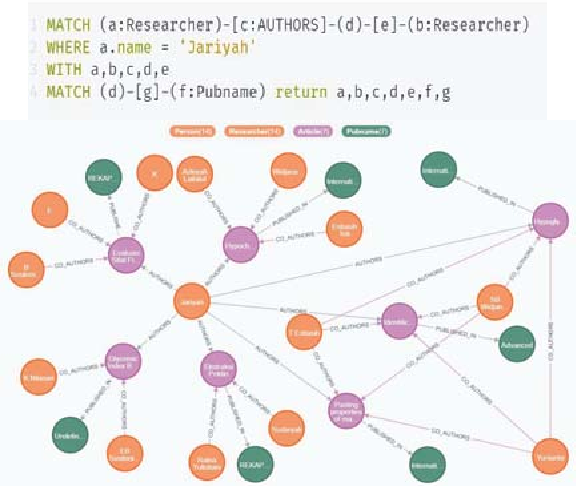
\includegraphics[scale=0.7]{Graficos/neo2.png}
    \caption{Caso 2 : Consulta Cypher}
    \label{fig:neo2}
    \end{figure}
\begin{figure}[H]
    \centering
    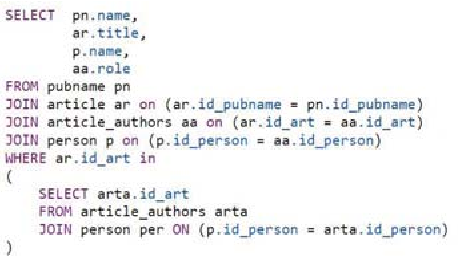
\includegraphics[scale=0.7]{Graficos/sql2.png}
    \caption{Caso 3 : Consulta SQL}
    \label{fig:sql2}
    \end{figure}

\subsection{Neo4j como la mejor opción para analístas}
La herramienta propuesta no solo brinda una gráfica iteractiva sino que además muestra las relaciones que posiblemente puedan llevarte a un objetivo que estes buscando.\\
Muestra toda la información correspondiente de cada nodo con su respectiva relación de la cual quisieras información y los posibles nodos que se vieran involucrados.
\begin{figure}[H]
    \centering
    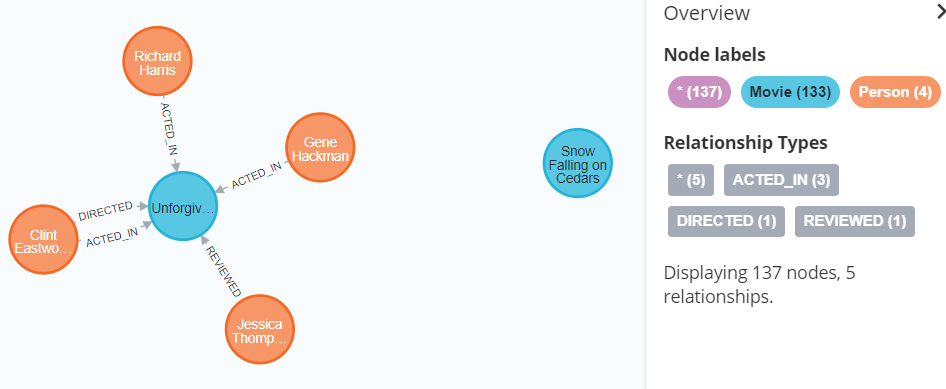
\includegraphics[scale=0.5]{Graficos/att.png}
    \caption{Nodo película Unforgiven con sus respectivas relaciones}
    \label{fig:att}
    \end{figure}
\subsection{Concytec como Información Valiosa}
En la técnica 2 pudimos evaluar como usan google schoolar como base de datos de investigadores para el mismo propósito de este papper, hacer que los universitarios tengan el mayor respaldo y asesoramiento posible de la manera mas accesible que puedan encontrar.\\
Concytec asi como google schoolar, brindan cierta información valiosa para un universitario el cual le permitirá elegir mejor a su asesor de acuerdo a lo que requieran. La segunda técnica mostró que es una necesidad realizar este tipo de propuestas para hacer que grupos de investigación como el que tiene concytec puedan ayudar a los demás.
\begin{figure}[H]
    \centering
    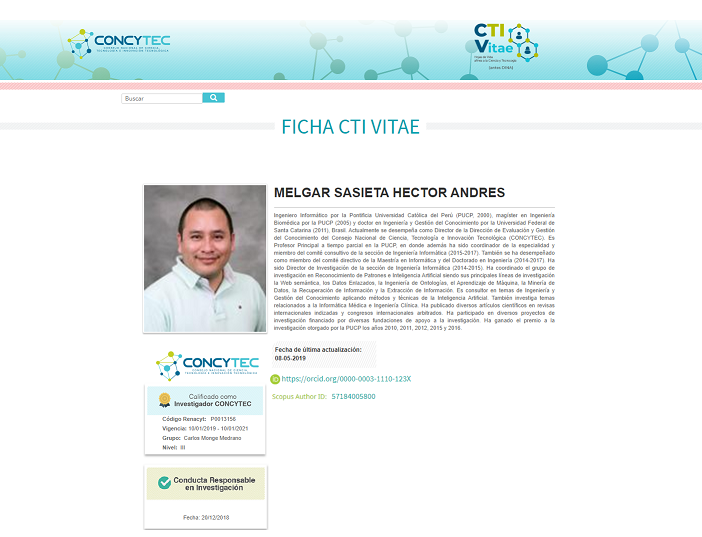
\includegraphics[scale=0.6]{Graficos/concytec.png}
    \caption{CV de profesor en la página de concytec}
    \label{fig:att}
    \end{figure}